% 
% Annual Cognitive Science Conference
% Sample LaTeX Two-Page Summar -- Proceedings Format
% 

% Original : Ashwin Ram (ashwin@cc.gatech.edu)       04/01/1994
% Modified : Johanna Moore (jmoore@cs.pitt.edu)      03/17/1995
% Modified : David Noelle (noelle@ucsd.edu)          03/15/1996
% Modified : Pat Langley (langley@cs.stanford.edu)   01/26/1997
% Latex2e corrections by Ramin Charles Nakisa        01/28/1997 
% Modified : Tina Eliassi-Rad (eliassi@cs.wisc.edu)  01/31/1998
% Modified : Trisha Yannuzzi (trisha@ircs.upenn.edu) 12/28/1999 (in process)
% Modified : Mary Ellen Foster (M.E.Foster@ed.ac.uk) 12/11/2000
% Modified : Ken Forbus                              01/23/2004
% Modified : Eli M. Silk (esilk@pitt.edu)            05/24/2005
% Modified : Niels Taatgen (taatgen@cmu.edu)         10/24/2006
% Modified : David Noelle (dnoelle@ucmerced.edu)     11/19/2014
% Modified : Roger Levy (rplevy@mit.edu)     12/31/2018


%% Change "letterpaper" in the following line to "a4paper" if you must.

\documentclass[10pt,letterpaper]{article}

\usepackage{cogsci}

%\cogscifinalcopy % Uncomment this line for the final submission 
%\twopagesummarysubmission % switch for two-page summary submissions so
                          % that they're never anonymized 


\usepackage{pslatex}
\usepackage{apacite}
\usepackage{float} % Roger Levy added this and changed figure/table
                   % placement to [H] for conformity to Word template,
                   % though floating tables and figures to top is
                   % still generally recommended!

\usepackage[none]{hyphenat} % Sometimes it can be useful to turn off
%hyphenation for purposes such as spell checking of the resulting
%PDF.  Uncomment this block to turn off hyphenation.


%\setlength\titlebox{4.5cm}
% You can expand the titlebox if you need extra space
% to show all the authors. Please do not make the titlebox
% smaller than 4.5cm (the original size).
%%If you do, we reserve the right to require you to change it back in
%%the camera-ready version, which could interfere with the timely
%%appearance of your paper in the Proceedings.

\usepackage{graphicx}

\title{Determinantal Point Processes for Memory and Structured Inference}



\begin{document}

\maketitle


\begin{quote}
\small
\textbf{Keywords:} 
mutual exclusivity; determinantal point process; memory;
variable-binding; compositionality; probabilistic models
\end{quote}

\section{Abstract}


Determinantal Point Processes (DPPs) are probabilistic models of repulsion, capturing the negative correlations between states.  Here, we show that a DPP operating in representation-space predicts inferential biases toward \textit{mutual exclusivity} that are commonly observed in word learning (mutual exclusivity bias) and reasoning (disjunctive syllogism) tasks. It does so without requiring explicit rule representations, without supervision, and without explicit knowledge transfer. The DPP attempts to maximize the total "volume" spanned by the subset of inferred code-vectors. Thus, when complex codes are constructed by re-using components, the DPP naturally favors binding previously un-used component representations (keys and values). We suggest that a bias toward maximizing volume in representation-space may exist to promote efficient memory encoding for retrieval. In support of this, we show that a DPP implements efficient "hashing", minimizing collisions without expanding the storage space required. Thus, the same mechanisms that promote rapid memory search may also underlie cognitive biases in structured inference.



\section{Background and Motivation}
Imagine that Tim and Tom are playing a Venezuelan board game called El Gocho. Tim won. What happened to Tom? Although you may not be certain, you don't need any more information to infer that it's likely that Tom lost. This is true despite the fact that you have no familiarity with the particulars of the game or the people. This reflects an inferential bias toward \textit{mutual exclusivity} (ME): the tendency to map individuals to 1/\textit{n} possible relational positions, and not to multiple positions at the same time. Although, in the El Gocho example, you came equipped with rich knowledge about the relational structure of \textit{games} that you could import, ME inferences have been observed surprisingly early in human development (Halberda 2003, Cesana-Arlotti et al. 2018), and in non-human species (Pepperberg et al. 2019). 

For example, a classic finding in developmental psychology is that, all else being equal, young children prefer to map a novel word ("zurp") to a novel referent (cathode-ray tube), rather than mapping many words to the same object, or many objects to the same word (Markman \& Wachtel, 1988; Halberda, 2003), a phenomenon known as the \textit{mutual exclusivity bias} (ME) in word-learning. At the same time, work in a different cognitive domain has found that pre-verbal infants assume that an individual object can not be in two places at the same time, and thus make inferences that resemble a formal disjunctive syllogism (\textit{A or B (but not both). Not A. Therefore, B}) (Cesana-Arlotti et al. 2018; See also Mody \& Carey, 2016)). 
 
 
Here, we argue that the class of ME inferences can be fruitfully considered as Determinantal Point Processes (DPP) operating over a representational space. DPPs are probabilistic models of repulsion between states: the more similar two states are, the less likely they are to co-occur (See Figure 1). DPPs originated in statistical physics to model the location of fermions at thermal equilibrium (Macchi, 1973), but have since been extended to other branches of mathematics and machine learning (Kulezsa \& Taskar, 2012). In machine learning, they have recently gained traction in the generation of sets of samples when sample \textit{diversity} is desirable, such as recommender systems looking to present a broad sample of item-types to users ((Kulezsa \& Taskar, 2012, Gillenwater et al. 2012; Chen et al. 2017). 

 \begin{figure}[h]
  \centering 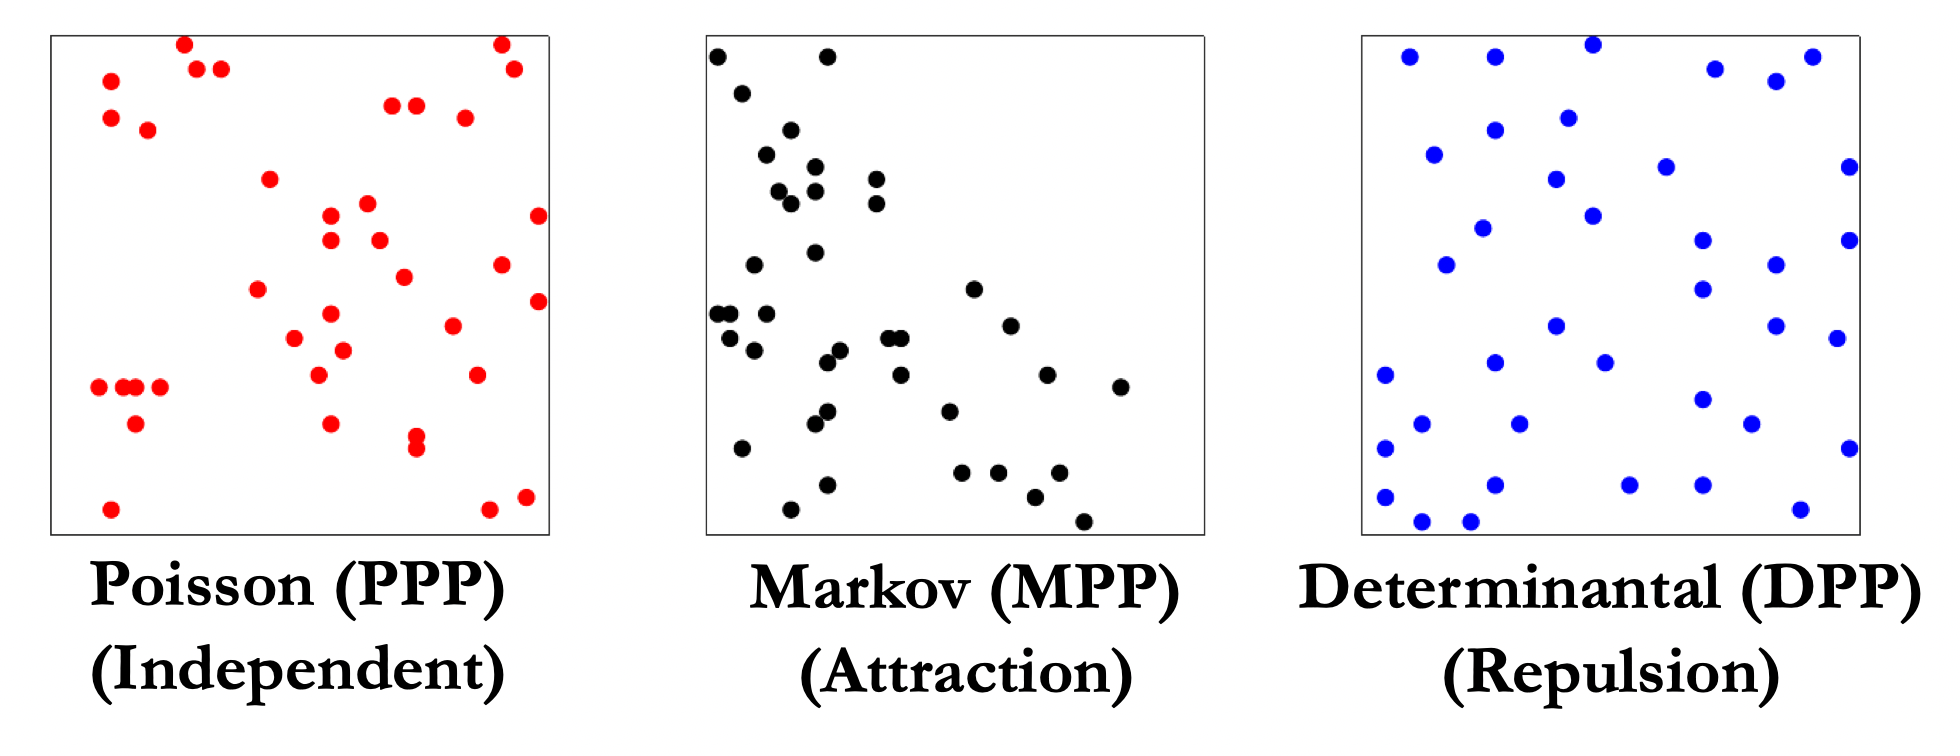
\includegraphics[width=1\columnwidth]{Figure1.png}
  \caption{Sampling in a plane for three types of point processes. PPP’s contain no relational information, and therefore, although likely to be spread across the space, can be susceptible to "clumping". MPPs, by contrast, carry relational information about the similarity between states, directly promoting such clumping. DPPs use the same similarity representation as MPPs, but, critically, \textit{repel} similar states, ensuring that samples are well distributed across the space.
}
\end{figure}

Here, we consider the inferential biases afforded by DPPs over a representational space. Specifically, we show (1) that when representations of possible combinations (e.g., word/object or location/object combinations) are compositions of re-usable codes, DPPs naturally predict the mutual exclusivity bias in word learning and reasoning by disjunctive syllogism. (2) We then show that, more generally, DPPs are generally advantageous to efficient memory retrieval, minimizing the collisions between possible data, by "repelling" similar keys. Finally, we (3) find that these ME effects are preserved when the initial encodings are mapped to high-dimensional, sparse, binary codes, like those known to exist in the hippocampus (McClelland, O'Reilly, McNaughton, 1995).

\section{Methods & Results}

We focus on two well-studied cases of mutual exclusivity in cognitive science: The "mutual exclusivity bias" in word learning (Markman & Wachtel, 1988; Merriman & Bowman, 1991; Halberda, 2003) and the ability to complete disjunctive syllogisms (Mody \& Carey, 2016; Cesana-Arlotti et al. 2018). We first describe the modeling approach in abstract terms, explaining the features that are common to both use-cases.

\subsubsection{DPP framework.}
Our model assumes a point process \textit{P} operating over a finite ground set \textit{Y} of discrete items. Here, the items are possible \textit{representations} (i.e., encodings) and more specifically, representations of particular key/value combinations (e.g., word/object or location/object combinations). The process defines a probability of selecting particular subsets (\textit{S}) of these combinations drawn from the ground set.

\[P (S \subseteq\ Y) = det (K _{S})\]

where \textit{K} is an \textit{NxN} positive semi-definite kernel matrix whose entries encode pairwise similarities between \textit{N} possible discrete states, where \textit{N} = \textit{m} keys X \textit{n} values. For all analyses reported here, we use a linear kernel, computed as a normalized inner product of each combination of the \textit{mXn} possible key/value vectors.

DPPs select a particular configuration of items so as to maximize the determinant (det) of the corresponding sub-matrix of \textit{K}, indexed by \textit{S}. (Macchi, 1973; Kulesza & Taskar, 2012). Thus, the central computation in current case is \(arg\ max \ _S\in_Y \ det(K _{S})\).

Geometrically, we can think of this determinant as the \textit{volume} spanned by the parallelpiped of the code vectors.  The more similar a set of vectors (small determinant), the less likely they are to co-occur in a set. The less similar the vectors (larger determinant), the more likely they are to co-occur in \textit{S}. This enables the modeling of repulsion between possible states; it is central to the current work and its ability to model aspects of higher-level cognition. 
 
 Here, the relevant representational states are concatenations of two types of code vectors corresponding to pre-factorized representations. These factors may be thought of as "keys" and "values", or alternatively "relations" and "content". Concretely, however, in the situations we explore, they are \textit{words} and their \textit{referents} in the ME-bias case, and \textit{spatial locations} and \textit{objects} in the disjunctive syllogism case. To generate the code for a possible combination, we simply concatenate vectors for the key/value components, keeping the ordering and codes consistent across uses, consistent with compositionality.\footnote{We note that, although this encoding framework is simple, it is motivated by empirical evidence concerning the nature and organization of the projections from the mammalian entorhinal cortex (EC) to the hippocampal sub-fields: a key circuit both for simple forms of reasoning (Dusek & Eichenbaum, 1997; Zeithamova et al., 2012) and memory. Specifically, a medial region of EC contains low-dimensional representations of the spatial structure of the environment, while a lateral region encodes sensory content (Behrens et al. 2018. See also Knierem et al. 2014). These separate representations are believed to then be bound together in the hippocampus in order to encode different structure/content combinations (Whittington et al. 2018).}


 Although finding the maximum a posteriori (MAP) subset in a DPP is  NP-hard (Ko et al. 2005, Kulezsa \& Taskar, 2012), there exist greedy methods that can effectively approximate it (Gillenwater et al. 2012, Han et al. 2017; Chen et al. 2018). However, here, we deal only with small cardinality domains, and thus are able to exhaustively search for the MAP in the possibility space. However, generating more plausible heuristic methods that can scale to larger spaces remains a focus for future work.  

\begin{figure*}[h]
  \centering 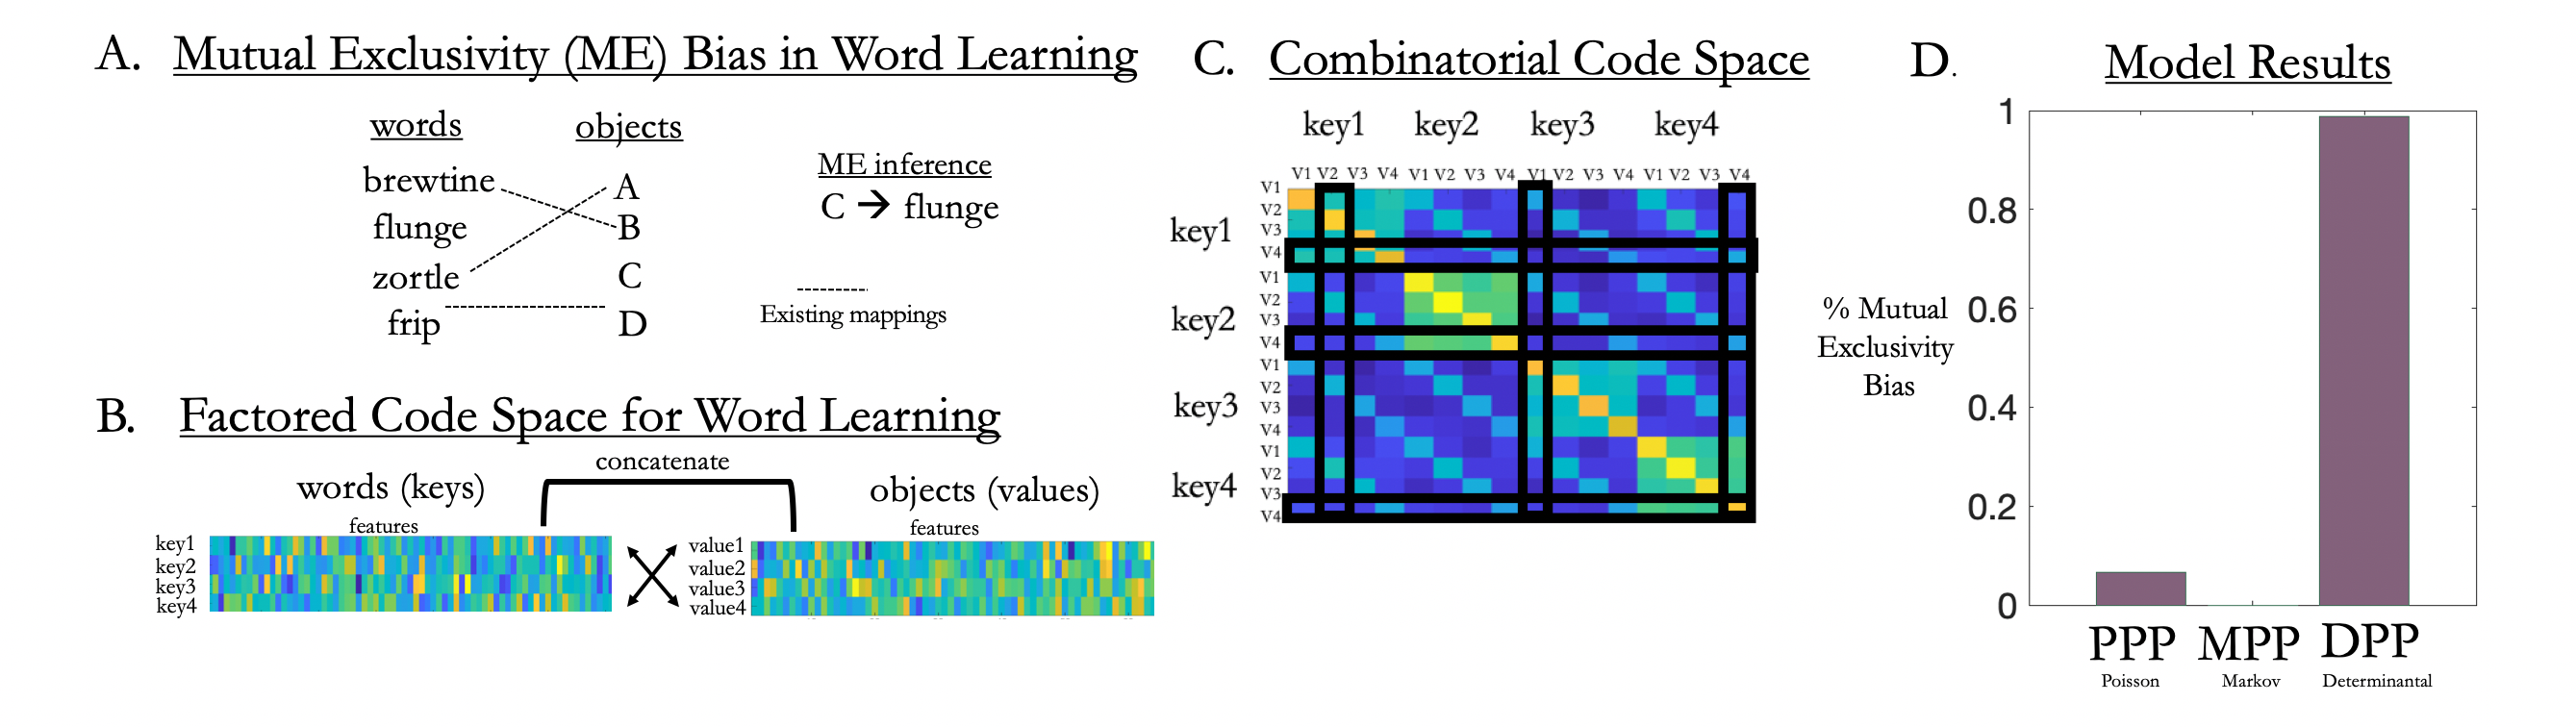
\includegraphics[width=\textwidth]{Figure2.png}
  \caption{\textbf{(A)}. Example of the word learning problem. The model’s task is to select a word/object mapping, conditioned on 3 existing associations. Humans tend to map the held-out word to the held-out object.
\textbf{(B)} shows the representations used by the models to guide inference. We assume separate, but combinable, codes for words (keys) and objects (values). The square matrix in \textbf{(C)} represents pairwise similarities between possible word/object combinations. Brighter colors reflect more similar combinatorial codes, darker colors less similar codes. Black bars across rows and columns reflect a hypothetical subset of word/object mappings, as in A.
\textbf{(D)} We evaluate the probabililty that the held-out word is mapped to the held-out object (mutual exclusivity bias) across 1000 simulations with different word/object codes. A DPP naturally selects the novel unused word and un-used object, exhibiting the mutual exclusivity bias.
}
\end{figure*}

Throughout, we compare the DPP to two alternative point process models. First, a Poisson Point Process (PPP), which assumes no similarity kernel \textit{K}, treating each item as independent. Here, we use \(P (S \subseteq\ Y) = \prod_ {i\in y} p_i \prod_ {i\notin y} \ (1-p_i)\), where \textit{p} is a flat prior across states. This is random uniform selection. Second, a generic Markov Point Process (MPP), which selects items based on the kernel \textit{K} used for the DPP, but selecting directly on the similarity scores of the sub-matrix, rather than its determinant. In this, the MPP over \textit{K} can be considered in opposition to the DPP, favoring items that are nearby in the code-space rather than far apart. Taken together, one can think of these three models as capturing the possibility of (a) random inference (PPP), (b) inference by similarity (MPP) and (c) inference by repulsion (DPP).


\begin{figure*}[h]
  \centering 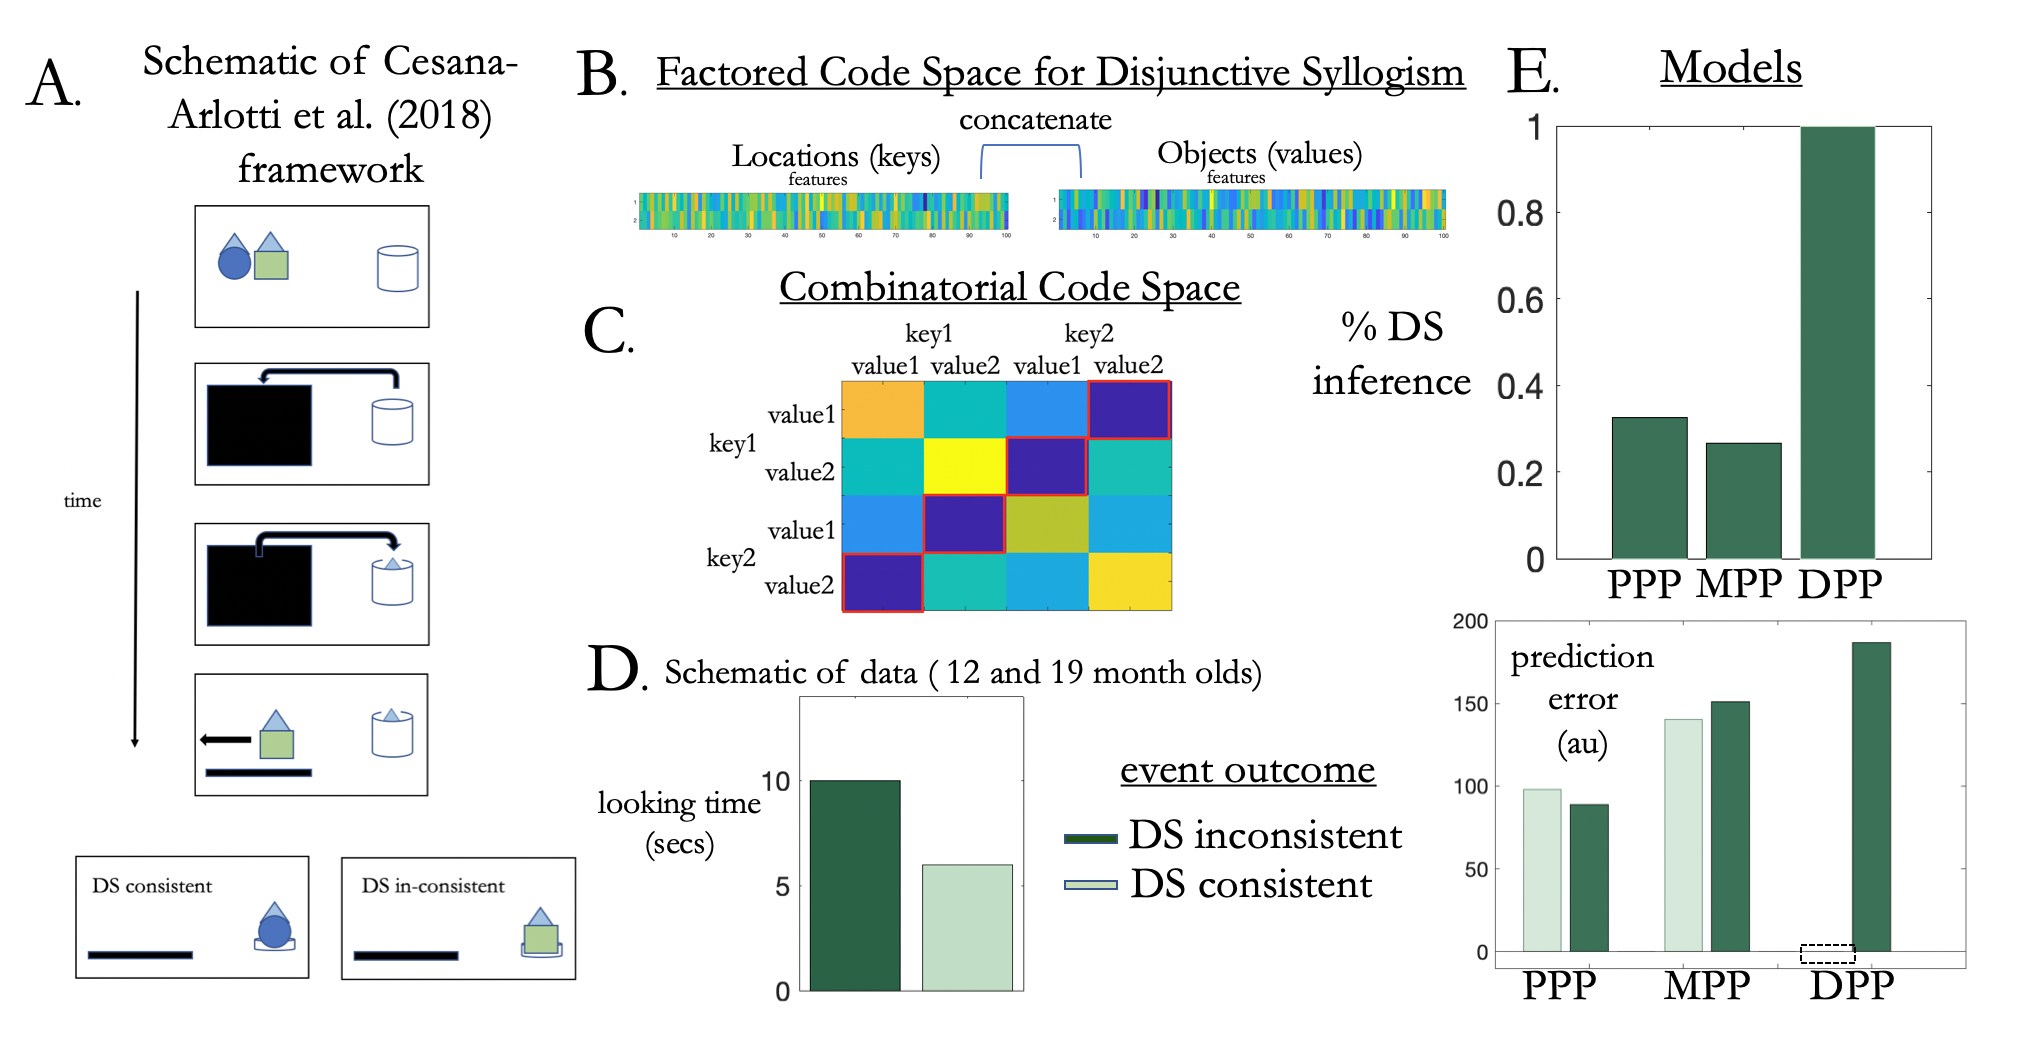
\includegraphics[width=\textwidth]{Figure3.png}
  \caption{\textbf{(A)}. Rendering of Cesana-Arlotti (2018)'s experimental paradigm, based on their Figure 1. \textbf{(B)}. To model this, we assume a factored space of object and location codes under consideration and \textbf{(C)} populate a square matrix with the pairwise similarities between possible object/location combinations (\textit{K}). We highlight in \textit{red} the items selected by  \(arg\ max \ _S\in_Y \ det(K _{S})\), conditioned separately on each combination that could be observed (the diagonal). The DPP reliably favors the combination that is most dissimilar (\textit{dark blue}) to the observed object/location combination (\textit{bright yellow}).  \textbf{(D)}. Cesana-Arlotti et al. (2018) found that infants exhibit increased looking time to DS-inconsistent cases (results schematically depicted here). \textbf{(E)} The DPP model naturally selects a combination of the un-used location and un-used object. If these infereces are used to generate prediction and compared against the DS-consistent and DS-inconsistent cases, the DPP exhibits greater prediction errors when the revealed object/location combination is DS-inconsistent, like pre-verbal infants.}
\end{figure*}

\subsection{Mutual Exclusivity Bias in Word Learning.}

 Here, we take the mutual exclusivity (ME) bias in word learning to be the empirical observation that, all else being equal, both young children and adults prefer to map a novel word to a novel referent, rather than mapping many words to the same object, or many objects to the same word (Markman \& Wachtel, 1988, Merriman \& Bowmnan, Halberda, 2003)). Here, we suggest that this inferential bias follows directly from the consideration of memory encoding as a Determinantal Point Process in a compositional space of representations. A learner that performs inference using a DPP over possible codes naturally repels similar codes in favor of more distinct ones, automatically favoring combinations of un-used words and objects.

We model a case involving 4 words and 4 objects, in which the learner has 3 extant word/object associations (See Figure 2a). Here, we are agnostic as to whether those associations were acquired in this particular episode, or whether they were brought to the episode. Words and objects are random code vectors, sampled from a multivariate Gaussian N(0,1). These codes are concatenated to form possible word/object combinations (See Figure 2c). We compute a linear kernel over the representations of these combinations, reflecting the covariance structure amongst the codes for different word/object pairs. The different point process models then select from the 13 remaining word/object combinations, conditioned on the 3 previous word/object combinations.



We ran 1000 simulations involving different random word and object vectors, and found that the DPP exhibits the mutual exclusivity bias 99.3 \% of the time. See Figure 2. As would be expected, the PPP model randomly selects from the 13 remaining possible conjunctions. The MPP prioritizes re-use of codes across instances (re-using a word to refer to multiple objects), given that its desideratum is to select combinations \textit{similar} to those already encountered. It has an inferential bias of "many-to-one".

Thus, when codes for combinatorial states are compositions of words and objects (keys and values), a simple algorithm that maximizes the volume spanned by the code vectors naturally produces a mutual exclusivity bias in the word learning process. Re-using either words or objects across different mappings in the same context works against maximizing the volume spanned by the vectors, as the same vector will contribute to multiple combinations. We further consider why such a bias toward volume-maximization might be beneficial to the organism below in the section entitled "DPP Hashing for Collision-Free Encoding". However, we first model a second cognitive phenomenon involving mutual exclusivity: the disjunctive syllogism.

\subsection{Disjunctive Syllogism.}

Our second example involves the ability to make inferences like those in a classical Disjunctive Syllogism (DS) (Mody \& Carey, 2016; Cesana-Arlotti et al., 2018; Pepperberg et al. 2019). Formally, a disjunctive syllogism starts with the representation of a disjunction (\textit{premise 1: A or B}), where 'or' is XOR (one or the other, but not both). Next, one acquires some piece of information (\textit{premise 2: not A}). Finally, a rule is applied to derive the conclusion, conditioned on the premises. (\textit{conclusion: Therefore, B}). Notably, young children (Mody \& Carey, 2016) including infants as young as 12 months (Cesana-Arlotti et al. 2018) and non-human animals (Pepperberg et al. 2019) all show aspects of this inferential ability. Here, we show that a DPP defined over the space of combinatorial representations predicts the key empirical pattern. 

For expository purposes, we focus here on the paradigm of Cesana-Arlotti et al. (2018)'s paradigm with pre-verbal infants. See Figure 3a for a schematic of a trial. A trial begins with two objects on a screen. Both are temporarily hidden behind an occluder, obstructing the objects from the infant's view. One object is then seen to be scooped out from behind the occluder, though the infant is unable to determine which of the two objects it was. The occluder is then removed revealing (e.g.,) object A.  The inference by disjunctive syllogism, of course, is that object B must therefore be the object in the bucket. Infants' expectations are assessed by measuring their looking time. If it is then revealed that the bucket contains object A, rather than object B (the "DS-inconsistent" condition), infants as young as 12 months old are surprised, evidenced by increased looking time relative to the alternative outcome in which object B is in the bucket ("DS-consistent" condition).

To model this, we assume 1x100 random code vectors sampled from a multivariate Gaussian (\mathcal{N}(0,1)) for each of two objects (values) and two locations (keys). We concatenate these to form a 4x200 matrix, in which the rows are compositions of possible object/location combinations, and the columns are random features. As above, we compute the covariance between each of the \textit{mXn} combinations, here obtaining a 4x4 kernel \textit{K} encoding the similarities between the codes for possible combinatorial states. For our analyses, we simulated 1000 different possible instances of random vectors, while also randomly selecting different superficial trial structures (e.g., that the DS-consistent combination was object A/location 1, object A/location2, object B/location1, objectB/location2). As expected, given one conjunction (e.g., object A in location 1), a DPP reliably selects the un-used object \textit{and} the un-used location (here, object B in location 2), as it maximizes the volume spanned by vectors encoding the combinations. See Figure 3. To more directly relate the models' inferences to the infant looking time data, we next computed the MSE between the object/location combination selected by the model and the code for the stimulus in the DS-consistent (low-surprise) and DS-inconsistent (high-surprise) conditions. As expected, the prediction error is high for the DPP model in the DS-inconsistent, and at zero for the DS-consistent condition. The MPP (similarity-based), and PPP (random) models do not predict this direction of the "surprisal" effect.


\subsection{DPP Hashing for Collision-Free Encoding.}

Why do these biases exist? One explanation is that natural selection has favored architectures that exhibit domain-specific ME biases because each confers an adaptive benefit in its domain (e.g., word learning, object tracking, reasoning by exclusion). Though we can not rule this out, we wish to suggest a more domain-general explanation: that ME is a consequence of an effective strategy for memory encoding. A DPP in code space helps promote rapid read out, minimizing collisions (interference) in the encoding. On this view, any representational domain that involves compositional encodings (re-using component representations to form complex combinations) could be expected to exhibit ME biases. 

To see the potential benefit to memory retrieval, it is instructive to consider data structures for "hashing" in computer science. A hash-function is a way of mapping from a datum to a unique index, such as a position in an array. Effective hashing seeks to avoid the time demands that are produced by sequential search techniques, which run in (O(\textit{n})) or binary search (which are O(\textit{log n})). Instead, a good hash-function enables (O(\textit{1})) access, in which readout time is invariant to  the number of items in the memory. This is a classic example of a space/time tradeoff (Sedgewick \& Wayne, 2011): If one is willing to use the resources to construct a vast array, data would never be mapped to the same position, and collisions would be minimized. However, this is costly in terms of space. By contrast, if there are relatively few locations, this would minimize space consumed, but would dramatically increase retrieval time, as one would have to search all the items in the particular location that is indexed. Hashing thus seeks to effectively navigate this trade-off, constraining both the size of the array that is needed (space), while also minimizing the amount of computation spent resolving collisions (time). DPPs in representational space manage this tradeoff.

Here, we consider a toy case in which locations in memory are indexed by a finite set of keys, and we are able to select a key for each datum. We compare "key-selection" for a PPP, MPP, and DPP where the latter two cases are defined over the similarity kernel for the space of key/value combinations in the dataset, as above. Figure 4 shows the results of 1000 simulations comparing the performance of these different models. DPP-based key selection (unlike PPP and MPP) ensures that particular keys will not be re-used, and thus each individual item will map to a unique location in memory (here, a region of the representational space). The probability of a collision in such a memory system is near 0 (Figure 4a). Moreover, we find that these infrequent collisions can be eliminated by use of Pearson correlation to compute K. Notably, this "collision-free" property is accomplished without dramatically expanding the size of the array, as the array size is no larger than the number of individual states we wish to encode (Figure 4b). A DPP-based hash algorithm, unlike random selection in a PPP, thus exploits the repulsive property to distribute codes evenly across the representational space.


\subsection{Towards a Hippocampal Model: DPPs over High-Dimensional Codes.}

\begin{figure*}[h]
  \centering 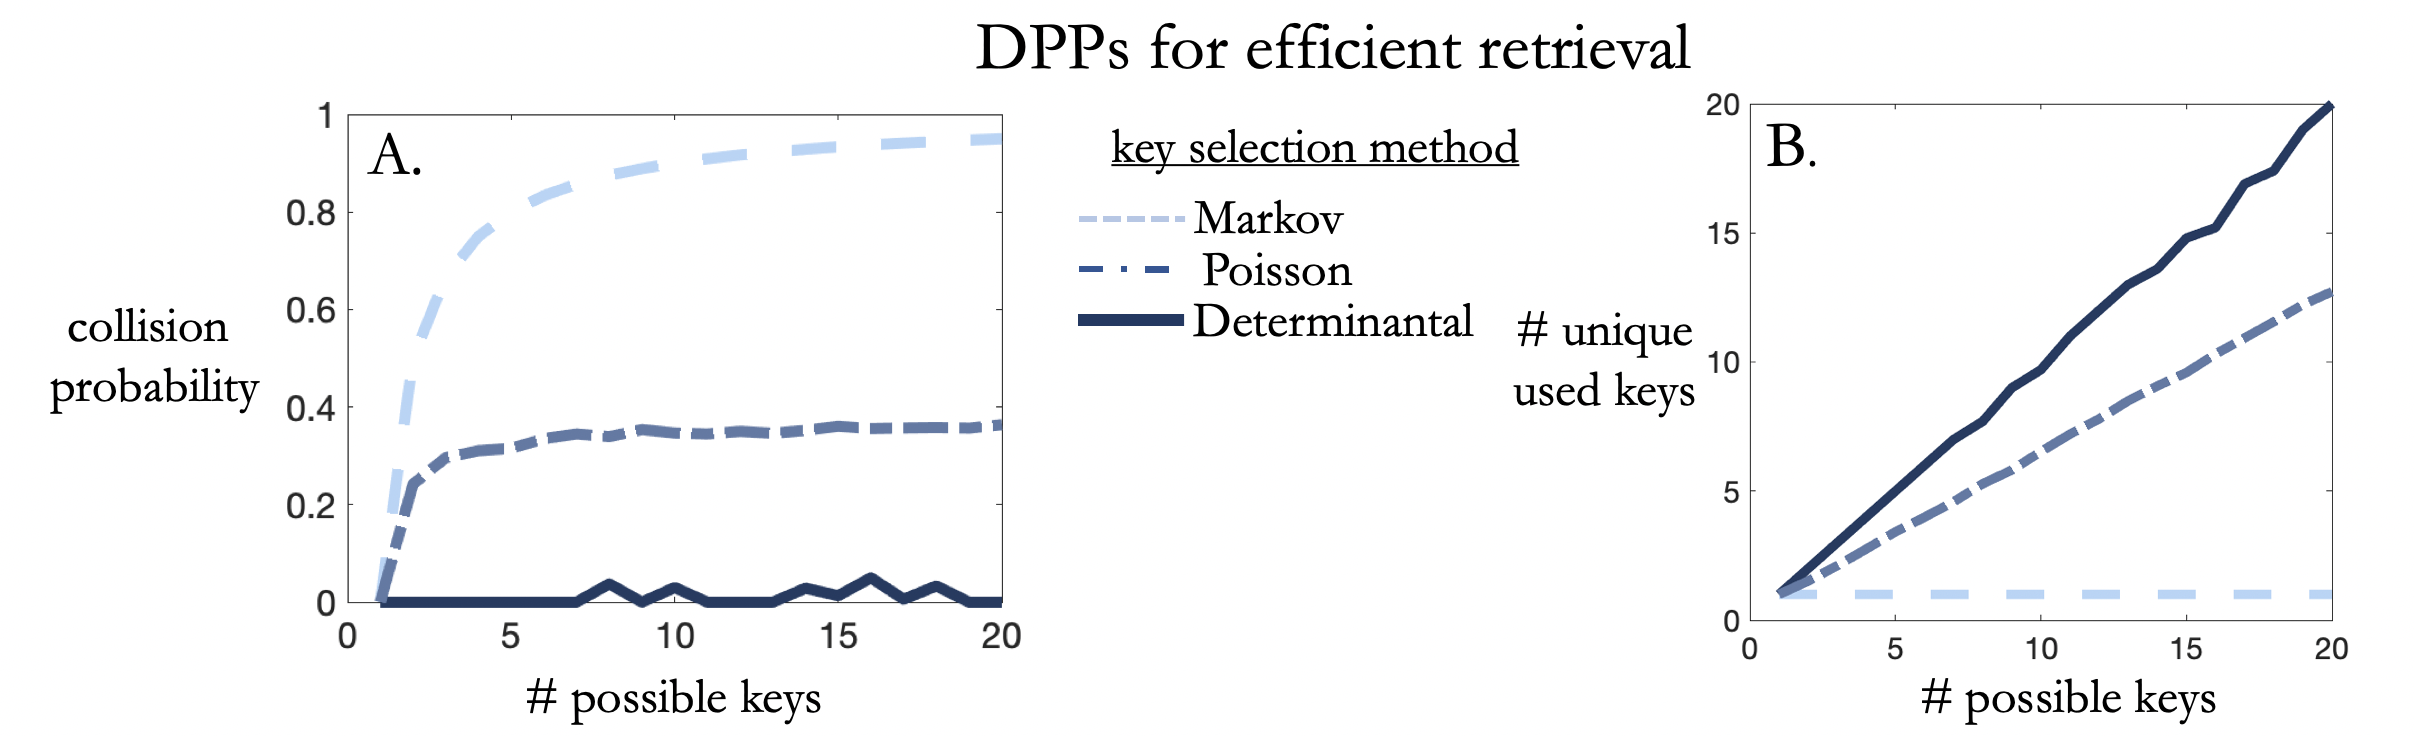
\includegraphics[width=\textwidth]{Figure4.png}
  \caption{DPP-driven codes enable efficient retrieval of unique items. We allow the keys of key/value pairs to be selected as a MPP, PPP, or DPP. DPPs \textbf{(A)} minimize collisions between items. They do so in virtue of \textbf{(B)} selecting un-used keys to maximize the volume spanned by the key/value code vectors, across the dataset. They thus efficiently manage the resource tradeoff between search time and storage space.}
\end{figure*}


We thus suggest the possibility that the ME bias stems from domain-general constraints on efficient memory retrieval. This raises the question: could the current DPP framework apply to representational spaces more likely to exist in the biological systems central to encoding and retrieval, like the hippocampus? Do the same biases exists over sparse, binary, high-dimensional codes? We assess this using a network of random linear projections from the key/value codes described above (which we'll now call "entorhinal cortex" or "EC") to a higher-dimensional "hippocampal" code space. We assume a network of 10,000 neurons that receive afferents from the key/value code units. We project the EC codes to the hippocampus, and apply a k-winner-take-all function to the output, rendering the hippocampal codes sparse, binary, and non-linear functions of the input. The sparsity of the resulting codes was also systematically varied, as was the density of connections between EC/hipp. (Figure 5). Once in the hippocampal space, we obtain the similarity kernel \textit{K} using normalized Hamming distances between the possible combinatorial states, and compute: \(arg\ max \ _S\in_Y \ det(K _{S})\),    as above.


Figure 5 shows the results when the determinants were computed in this higher-dimensional hippocampal space. Notably, the results are qualitatively similar to the DPP computation over the cortical codes themselves (Figure 2 \& 3). Sparse, binary codes computed as random projections of key/value (entorhinal cortex) pairs thus preserve the ability to use DPPs for inductive inference, showing the same ME bias. A classic finding in computer science shows that random projections preserve the similarity relationships between items, both when the dimensionality is reduced (Johnson-Lindenstrauss), and also \textit{expanded} Dasgupta et al. (2017). Given that we compute the determinant over the similarity kernel \textit{k}, it stands that these random projections to a high-dimensional space are also, \textit{(ipso facto) volume} preserving, which we see evidence for here.



\begin{figure}[h]
  \centering \includegraphics[width=1\columnwidth]{figure5.png}
  \caption{The same inferential biases for \textbf{(A)} word learning and \textbf{(B)} disjunctive syllogism cases are preserved when the DPPs operate over sparse, binary high-dimensional codes, like those of the hippocampus. }
\end{figure}

\subsection{Discussion}
 We have shown that Determinantal Point Processes (DPPs)--probabilistic models of the negative interactions between states--predict observed biases in structured inference. Specifically, inferential biases toward (a) mutual exclusivity in word learning (Markman \& Wachtel, 1988; Halberda, 2003) and (b) completion of disjunctive syllogisms (Mody \& Carey, 2016; Cesana-Arlotti et al., 2018) arise naturally from a DPP that favors the combination of un-used representations.


This framework does not require that the cognitive system have explicit representations of rules, receive direct supervision, or have mechanisms for transferring knowledge between domains, putting ME biases well-within the cognitive reach of young children, pre-verbal infants and non-human species that may be lacking in relevant experience, cortical machinery, or both (See Mody \& Carey, (2016) for related discussion regarding disjunctive syllogism in young children).

Instead, we suggest that the central driver may be the promotion of an efficient memory system. Maximizing the volume spanned by the vectors in code space promotes retrieval by minimizing interference ("collisions"). This is closely related to classic ideas regarding \textit{pattern separation} (Marr, 1971; Treves and Rolls, 1995; O'Reilly & McClelland, 1994), in which similar codes are projected into a high-dimensional space where the probability of collisions is low. One can view the DPP as an extension of this thinking. Although the DPP doesn't 
\textit{require} an expansion of dimensionality in order to reduce collisions (See Figure 4b) it can, none the less, tolerate expansion, even exhibiting the same inferential biases as when computed in lower-dimension (See Figure 5).

We note two potential disadvantageous to using a DPP for hashing, however. First, the DPP is inherently relational, and thus requires knowledge of the dataset under consideration. This may be provided by incorporating canonical representation, shared across domains. However, in general, the DPP is better equipped to store and reason about the relations between items \textit{within a particular context}. Second, computing the determinant is costly (either \textit{O(n3} or \textit{O(!)}, depending on the approach) Although this difficulty of computing the hash-function likely limits the DPP's use in application, this exponential increase in computational complexity provides an intriguing connection to the non-linear set-size effects in the working  memory literature (Miller, 1957; Luck \& Vogel, 1997). One possibility is that capacity limits that appear to stem from a fixed number of "slots" may instead owe to the scaling of the complexity of computing the determinants necessary to encode an increasing number of individual/location combinations. A better understanding of how DPPs related to the various memory systems, as well as the architecture of entorhinal/hippocampal systems is a topic of ongoing work.

\nocite{behrens2018cognitive}
\nocite{cesana2018precursors}
\nocite{chanales2017overlap}
\nocite{dasgupta2017neural}
\nocite{dusek1997hippocampus}
\nocite{halberda2003development}
\nocite{gillenwater2012near}
\nocite{ko1995exact}
\nocite{knierim2014functional}
\nocite{kulesza2012determinantal}
\nocite{luck1997capacity}
\nocite{markman1988children}
\nocite{10.2307/2417171}
\nocite{merriman1989mutual}
\nocite{miller1956magical}
\nocite{mcclelland1995there}
\nocite{mody2016emergence}
\nocite{o1994hippocampal}
\nocite{quine2013word}
\nocite{treves1994computational}
\nocite{whittington2018generalisation}
\nocite{zeithamova2012hippocampus}


%\nocite{ChalnickBillman1988a}
%\nocite{Feigenbaum1963a}
%\nocite{Hill1983a}
%\nocite{OhlssonLangley1985a}
% \nocite{Lewis1978a}
%\nocite{Matlock2001}
%\nocite{NewellSimon1972a}
%\nocite{ShragerLangley1990a}


\bibliographystyle{apacite}

\setlength{\bibleftmargin}{.125in}
\setlength{\bibindent}{-\bibleftmargin}

\bibliography{CogSci_Template}

More generally, DPPs offer a number of potential benefits to cognitive models that require repulsion between states. First, they permit exact inference. Second, they are computable with linear algebra, and thus, \textit{prima facie} neurally plausible.


\footnote{See Chanales et al. (2017) for intriguing fMRI evidence of "repulsion" in hippocampal codes, in which similar states have more dissimilar representations.}

\end{document}
